% Archivo generado automáticamente con los problemas
\section*{Problems}
Sección: 29_Weak_interactions
Páginas: 633-634
Contenido:
29.1 The dominant production mechanism for Higgs bosons at LEP was e+e−→ZH.
Calculate the total cross section for this process at tree-level in the Standard Model.
How many 100 GeV Higgs bosons would there have been when LEP ran at
206 GeV?

29.2 e + e−→hadrons in the Standard Model.
(a) Calculate the rate for the total cross section σtot(e + e−→hadrons) in the
Standard Model at tree-level including both Z-boson and photon contributions
and their interference. The contribution using photons alone was calculated in
Section 26.3.
(b) Calculate σtot at 1-loop.
(c) Plot the total cross section as a function of center-of-mass energy showing sepa-
rately the photon contribution, the Z-boson contribution, and their sum. Plot also
the sum ignoring interference between the Z-boson and photon contributions.
When can interference be ignored?

29.3 Higgs decays.
(a) Calculate the rate for H →b¯b in the Standard Model.
(b) Calculate the rate for H →gg in the Standard Model. The dominant contribu-
tion to this comes from a triangle loop diagram involving top quarks.
(c) Calculate the rate for H →γγ in the Standard Model. Include contributions
both from top loops and from loops of W bosons.
(d) Plot the branching ratios for H →b¯b, H →gg and H →γγ as a function of
Higgs mass.

29.4 Partial wave unitarity.
(a) Calculate the matrix element for longitudinal W +
L W −
L →W +
L W −
L scattering in
the Standard Model.
(b) Show that the high-energy behavior of this matrix element is reproduced using
the Goldstone boson equivalence theorem.
Problems
615
(c) Does this give a stronger unitarity constraint than the one using W +
L ZL →
W +
L ZL scattering?

29.5 Figure 29.2 includes a number of experimental constraints on the CKM matrix.
(a) The parameter εK is what we were calling ϵ in Section 29.5.2. Why do the
curves marked εK have the shape they do? That is, what combination of CKM
elements is εK sensitive to?
(b) What could you measure to produce the curves marked Δmd or |Vub|?

29.6 Show that with general Dirac and Majorana mass matrices, there are three phases in
the PNMS matrix, while if the mass matrix is purely Dirac, there is only one. How
many phases are there if the masses are purely Majorana?

29.7 Neutrino oscillations.
(a) Neutrinos are produced in the Sun predominantly through the reaction p + p +
e−→d + νe. What is the momentum of the neutrinos produced this way?
(b) Consider a two-neutrino flavor system. The mass eigenstates evolve in time as
|ν1⟩= e−iE1t
cos θ|νe⟩+ sin θ|νμ⟩

,
(29.117)
|ν2⟩= e−iE2t
−sin θ|νe⟩+ cos θ|νμ⟩

,
(29.118)
where θ is the mixing angle. Show that the probability of finding a solar neutrino
as an electron neutrino after a time T is given by
P = 1 −sin2(2θ) sin2 (E2 −E1)T
2
.
(29.119)
(c) Take the non-relativisitic limit E ≫mν to show that the probability of finding a
solar neutrino with energy E as an electron neutrino at a distance L is given by
P = 1 −sin2(2θ) sin2 Δm2L
4E
.
(29.120)
(d) How far should you put your detector from a reactor producing ∼4MeV
neutrinos assuming Δm2 = 7.5 × 10−5 eV2 to see the largest effect?

29.8 Show that when you integrate out the right-handed neutrinos in Eq. (29.63), a
dimension-5 operator like that in Eq. (29.65) results. What is the exact relationship
between Mij and 7
Mij?

29.9 Show that when multiple generations are rotated, then the θ angle shifts by
arg det

R†L

.

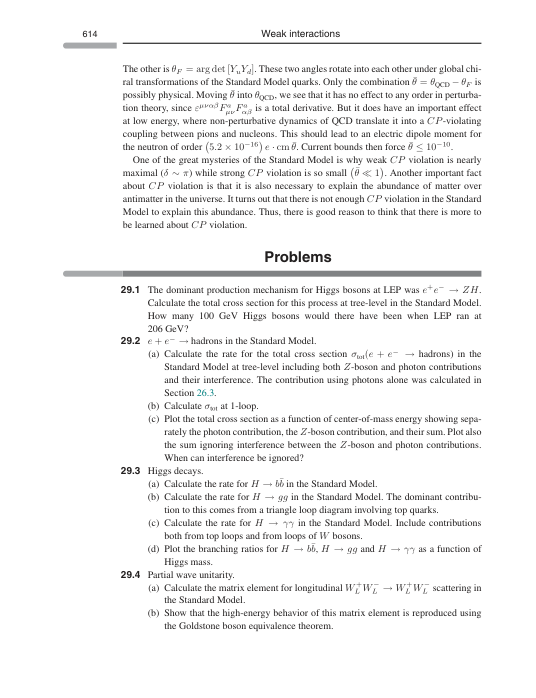
\includegraphics{./figs/29_Weak_interactions_page_634.png}

---

